\section{Literature Review}

\subsection{Motor-sport Aerodynamics}
In 1949 Ludwig Prandtl stated, "The term aerodynamics is generally used for problem arising from flight and other topics involving the flow of air \cite{Anderson2007FundamentalsJr.}". By definition, Aerodynamics is one of the branch in physics which concern and study the interaction of a body and fluid flow stream \cite{Scibor-Rylski1984RoadAerodynamics}. The forces' magnitude and direction occur on a body is a result of the flow interaction which depends on several variables. Some fundamental variables in aerodynamics include flow velocity, temperature, pressure, and density, which further describe the flow physics and characteristic. Drag and lift are the greatest consideration in race-car aerodynamic which will be discussed further on next subsection on this paper.

\noindent Aerodynamics is generally classified into external (flow around  the body) and internal (flow inside the body). This paper will focus on external aerodynamics which focus on the force generation due to the air-stream behaviour around the body of interest. In the automotive industry, external force plays an important part since the overall performance of the car is dependent on the aerodynamics forces created which significantly influence and improve the vehicle shape to its aerodynamics advantage \cite{Scibor-Rylski1984RoadAerodynamics}. Some of the aerodynamics consideration to vehicle's shape influence include large downforce generation, downforce balance between from and rear tyre, and drag minimisation. Table \ref{Table1} shows the effect of downforce to a racing car's acceleration, it can be seen that downforce significantly improve the acceleration time by -1.06 seconds, rate of acceleration by 4.5 $m/s^2$, and power by 124 kilowatt. 

\begin{table}[!ht]
\caption{\label{Table1} Aerodynamic downforce effect of a racing car acceleration \cite{Scibor-Rylski1984RoadAerodynamics}.}
\vspace{-5mm}
\begin{center}
 \begin{tabular}{||c| c| c ||} 
 \hline
 Variables & With Downforce & Without Downforce \\ [0.5ex] 
 \hline\hline
 Time from 0 to 160 $km/h$ & 5s & 6.06s \\ 
 \hline
 Rate of acceleration at 44 $m/s$ & 10.02 $m/s^{2}$ & 5.52 $m/s^2$ \\
 \hline
 Power transferred at 44 $m/s^2$ & 353 kW & 229 kW  \\
 \hline
\end{tabular}
\end{center}
\end{table}

\noindent Queen's Formula Racing has started to focus on aerodynamics since 2016. Previous students have attempted to analyse the previous QFR car including undertray to optimise its overall performance.  This paper will solely focus on external aerodynamics to understand the flow behaviour of a QFR undertray and its force generation, which then the analyses are used for geometry consideration of the aerodynamic undertray.

\subsection{Aerodynamics Fundamental}
To fully understand the flow physics and behaviour of the aerodynamic undertray, there are several fundamental understanding or terminologies of aerodynamics which needs to be firstly understood.

\subsubsection{Flow Types}
The main characteristic of a liquid is the molecule ability to freely move around the space. The movement of liquid molecule to another point in space also requires energy, mass, and momentum to be transferred with it. In this occasion the "transfer phenomena" occurred, where the molecules introduced to viscosity (friction), thermal conduction, and mass diffusion \cite{Anderson2007FundamentalsJr.}. The flow that shows the indication of "transfer phenomena" can be called as viscous flow. On the other hand, the flow condition where the "transfer phenomena" does not occur is known as inviscid flow.

\noindent Some flow such as streamline far from wall can be represented by the inviscid flow. But to capture the aerodynamic behaviour between two near moving wall such an undertray, the viscous flow plays a crucial factor. The shear stress near wall boundaries is occurred by the presence of viscosity which become one of the major source in drag, as well the presence of viscosity allows us to capture flow separation on the high incident geometries. Viscous effect is important consideration in the analysis where the body of interest is purposely designed to generate aerodynamic forces due to the flow such as, airfoil and undertray.

\noindent Another important properties in aerodynamics is density ($\rho$). Compressibility on a flow is fully dependant on the the state of its density at certain speed. Incompressible flow can be referred to a flow with constant density throughout, which usually happen at the region of Mach number less than 0.3. In contrast the region of Mach greater than 0.3 is known as compressible flow where density is variable\cite{Anderson2007FundamentalsJr.}.

\subsubsection{Reynolds Number}
%talk about reybold Number as well how it affects the flow characteristic
Reynolds number is a dimensionless ratio of inertial and viscous forces which used to classify the probability of flow being laminar or turbulent\cite{Rehm2008SituationalMPD}. Mathematically, Reynolds Number can be expressed as:

\begin{equation}
Re = \frac{\rho v d}{\mu} = \frac{inertial force}{viscous force}
\end{equation}

\noindent For low Reynolds number, the flow can be categorised as laminar where the molecules move in a regular, smooth, steady, and no mixing between layer occurred\cite{Obidi2014TheoryVehicles}. In contrast the turbulent flow usually occur at high Reynolds number where the fluid particles travel in random and irregular attitude in which break up the streamline. When the flow is changing from laminar to turbulent, this flow is called transition region. Figure \ref{fig:2} shows the difference in laminar flow with transition to turbulent region near the wall. 

\begin{figure}[!h]
    \centering
    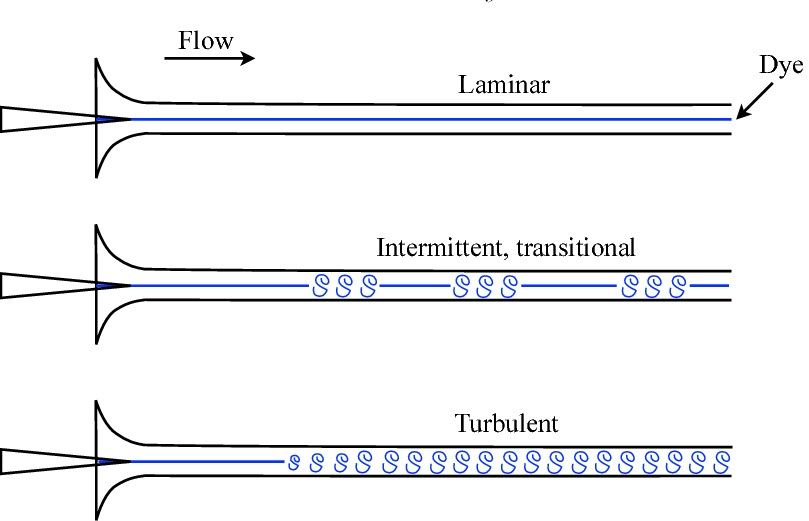
\includegraphics[scale=0.3]{Figures/laminar_turbulent_difference.jpg}
    \caption{Illustration of difference between laminar, transition, and turbulent flow in a pipe \cite{D.BARKLE2016TheoreticalPipe}.}
    \label{fig:2}
\end{figure}

\subsubsection{Boundary Layer}
Boundary layer is the referred as the viscous flow region adjacent to the body surface \cite{Anderson2007FundamentalsJr.}. The layer of air stream surrounding the body at a distance near the wall move with various relative speed, therefore this create a velocity gradient ($\frac{\partial V}{\partial y}$) which the speed on the surface is zero (non-slip condition) to local velocity outside the surface layer \cite{Scibor-Rylski1984RoadAerodynamics}. This layer is also referred as boundary layer. Figure \ref{fig:3} show the development of boundary layer on a flat plate, it started with laminar flow which transitioned into turbulent flow with formation of eddies in it.

\begin{figure}[!h]
    \centering
    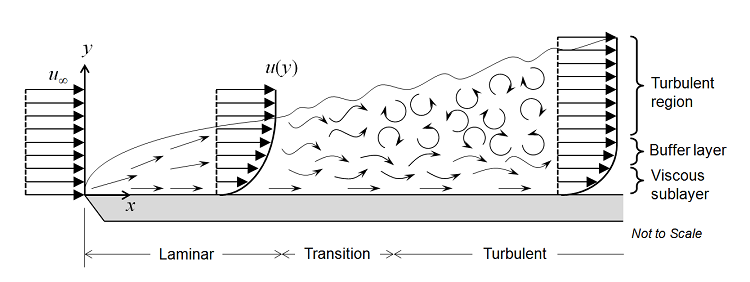
\includegraphics[scale=0.6]{Figures/BL_laminar_turbulent.png}
    \caption{The difference of boundary layer along flat plat \cite{Frei2017WhichApplication}.}
    \label{fig:3}
\end{figure}

 
\noindent From figure \ref{fig:3}, it can be seen that there are two main types of boundary layer flow: laminar and turbulent. Laminar is demonstrated close to the leading edge where the fluid travel smoothly which shows a low velocity gradient and low friction near the wall. When the velocity gradient increases and the friction on one layer to another is significant, the flow can be stated as turbulent \cite{Scibor-Rylski1984RoadAerodynamics}. This can be indicated with irregular and random fluid movement with presence of eddies. Boundary layer is important due to its ability in producing drag due to skin friction. When the local velocity increases, the velocity gradient $(\frac{\partial V}{\partial y})_{y=0} $ and shear stress near the wall ($\tau_w $) also increases with the overall drag.

\noindent It has to be noted that turbulent flow and separated flow are related but different flow characteristic. Flow separation occurs where the air stream effect is reversed when the surface geometry is curving away . When the air stream slows down, the pressure gradient inverses which create an adverse pressure gradient and then cause a thickening in boundary layer \cite{Scibor-Rylski1984RoadAerodynamics}. The condition let the shear stress (friction) and adverse pressure gradient bring the molecules at the very near of the wall come to stop. At this stage the boundary layer separates  and create a region of reversed flow. This condition is illustrated on figure \ref{fig:flow separation}.

\begin{figure}[!ht]
    \centering
    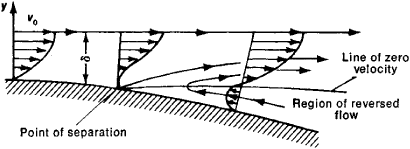
\includegraphics[scale= 0.8]{Figures/flow_separation.png}
    \caption{Illustration of separated flow formation along curved body \cite{Anonymous1979SeparationDictionary}}
    \label{fig:flow separation}
\end{figure}

\subsubsection{Bernoulli Equation \& Venturi Effect}
Bernoulli equation is another important mathematical analysis that analyse the relationship between the flow speed and pressure, this is a fundamental theory of the aerodynamic undertray. The equation can be expressed as:
\begin{equation}
   \underbrace{p}_\textrm{Pressure Energy} + \underbrace{\frac{1}{2} \rho V^{2}}_{\substack{\text{Kinetic Energy} \\ \text{per Unit Volume}}} + \underbrace{\rho g h}_{\substack{\text{Potential Energy} \\ \text{per Unit Volume}}} = constant
    \label{eq:bernoulli}
\end{equation}
Equation \ref{eq:bernoulli} clearly states the relationship between speed and pressure where the flow's density is assumed constant. This states that pressure is inversely proportional to the air speed, therefore increase in velocity has to be accompanied with reduction in pressure and vice versa. This strongly correlated to the downforce generation of an undertray, flow acceleration on the bottom of a car will reduce the pressure, hence high downforce.

\noindent The underbody of a race car can be modelled as a Venturi tunnel where the undertray the airflow goes into area reduction then expanded at the rear which illustrated in figure \ref{fig:venturi_tunnel_car}. The purpose of this shape is to accelerate the flow underneath the body then slowly expanded at the rear diffuser. The continuity formula $\rho AV = constant$ stated the reduction in underbody cross sectional area increases the velocity, hence decreases the pressure (from equation \ref{eq:bernoulli}).

\begin{figure}[!ht]
    \centering
    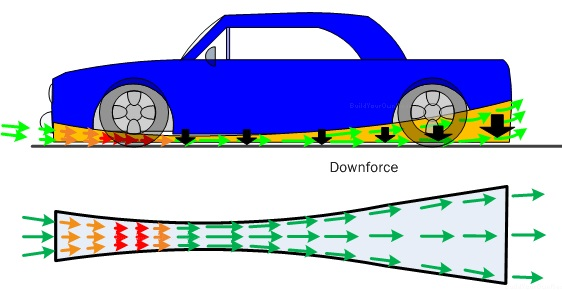
\includegraphics[scale=0.8]{Figures/venturi_tunnel.jpg}
    \caption{Venturi tunnel modelling of an automotive underbody \cite{Anonymous2020RaceDesign}.}
    \label{fig:venturi_tunnel_car}
\end{figure}
\noindent It is worth to be noted that this simplification only applied on ideal condition where the air mass is fully conserved throughout the undertray. In real-life condition, there are some air leakage on the side and creates a corner vortices which greatly affect the overall car performance. The rule of thumb for designers is to maximise the cross-sectional area reduction on the inlet and area expansion on the rear, due to viscosity, this case will not be possible. High area reduction on the inlet will accelerate the flow but also proportional to its drag and high diffuser area (outlet angle) will create flow separation which reduce the downforce and create a significant wake at the rear of the car, hence higher drag. To achieve an optimised underbody geometry, broad variables has to be broadly and deeply analysed to identify each of its effect to the aerodynamic force.


\subsubsection{Aerodynamic Forces}
%due to to flow around the body there are some generation of force occurred etc
Forces optimisation which generated by the aerodynamic flow are the main goal of this paper. The Bernoulli Equation from section 2.2.4 indicated that the flow pattern around a body produces pressure distribution over the surface \cite{Scibor-Rylski1984RoadAerodynamics}, which means integrating the pressure over the body surface will result in total forces caused by the flow around the body. The general force of a body can be expressed as:
\begin{equation}
    F = qSC_f
\end{equation}
Where $C_f$ is a dimensionless coefficient which fully dependant on the shape of the body \cite{Scibor-Rylski1984RoadAerodynamics} and $S$ is the area on which the surface the force of a body. In a drag analysis, the surface is the frontal area of a body which imposed the flow velocity (illustrated on figure \ref{fig:Force direction and frontal area} right). On the other hand, the lift analysis will require the area of the lift generator (e.g. undertray, inverted wing, or car wetted-surface).

\begin{figure}[!h]
\begin{center}
%    
  \begin{subfigure}[b]{0.4\textwidth}
    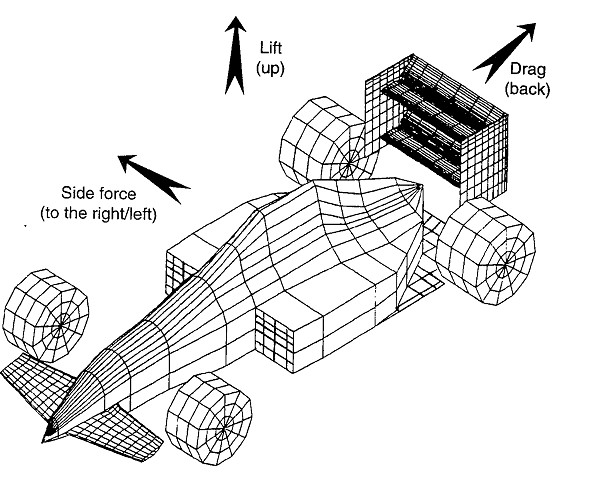
\includegraphics[scale=0.4]{Figures/race_car_forces.jpg}
  \end{subfigure}
  %
  \begin{subfigure}[b]{0.4\textwidth}
    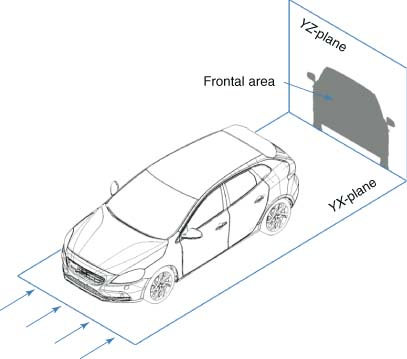
\includegraphics[scale=0.8]{Figures/frontal_area.jpg}
  \end{subfigure}
%  
  \caption{Force direction acting on a race-car(left) and representation of frontal area of an automotive body(right)\cite{Sebben2014FundamentalsDesign}.}
    \label{fig:Force direction and frontal area}
\end{center}
\end{figure}
\noindent There are three main forces acting on a car body: lift, drag, and side force. Figure \ref{fig:Force direction and frontal area} left illustrate the direction of forces acting on a car. Due to the function of undertray, this paper will only focus on the generation and optimisation of lift and drag.

\paragraph{Lift (downforce)}
%definition of lift
Lift is an applied force due to the pressure difference on a body which acts vertically and perpendicular to the drag force \cite{Scibor-Rylski1984RoadAerodynamics}. It can be mathematically expressed as:
\begin{equation}
    L = \frac{1}{2}\rho U^2 S C_L
\end{equation}
%lift in race car 
It is important in motor-sport industry that a race car produce as much downforce (negative lift) with the least drag possible. In aviation field, the aerofoil generate positive force to lift the aircraft from the ground, on the other hand, lift on race car used to increase the tyre grip by using an inverse aerofoil concept which produce a negative force. This consideration is due to the significant improvement in road handling and tyre grip which enables higher cornering speed, acceleration, and braking \cite{Barnard1997RoadIntroduction}.


\paragraph{Drag}
Drag is a force that work against the intended direction of a body which manifest in form of friction or pressure\cite{Obidi2014TheoryVehicles}. The drag force direction always follows the flow velocity of the car motions. Drag force can be mathematically expressed as:
\begin{equation}
    D = \frac{1}{2}\rho U^2 S C_D
\end{equation}
In case of formula student car, the flow travels around the car can be assumed as stokes flow (low Reynold number flow) which stated that drag is directly proportional to the viscosity, velocity, and size \cite{Obidi2014TheoryVehicles}. If the viscosity of air can be assumed as constant in the analysis, therefore the only variable which could be modified to reduce the drag is the size or geometry of the body. It has to be noted that race-car drag also divided into 5 different type of drag \cite{Kelly1964AerodynamicsEngineers}: form drag, lift drag, surface drag, interference drag, internal flow drag.

\subsection{Aerodynamics Undertray}
Undertray is an aerodynamics device that is attached to the underside of a race car that take advantages of the aerodynamic flow to decreases the pressure and increase the downforce significantly. Undertray has become an important part in motor-sport industry due to its ability to produce 45\% of car's downforce \cite{Katz1995RaceSpeed}. A typical undertray consist of a nozzle (inlet), floor section (throat), and diffuser (outlet).  Figure \ref{fig:underbody} shows an example of simple undertray of a formula car.

\begin{figure}[!ht]
\begin{center}
%    
  \begin{subfigure}[b]{0.4\textwidth}
    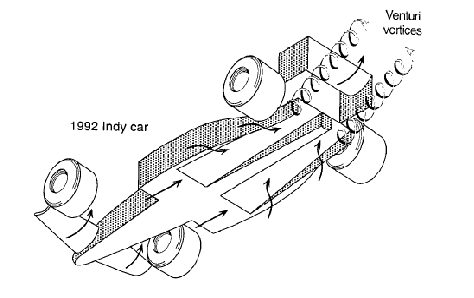
\includegraphics[height=4.8cm]{Figures/underbody.PNG}
  \end{subfigure}
  %
  \begin{subfigure}[b]{0.4\textwidth}
    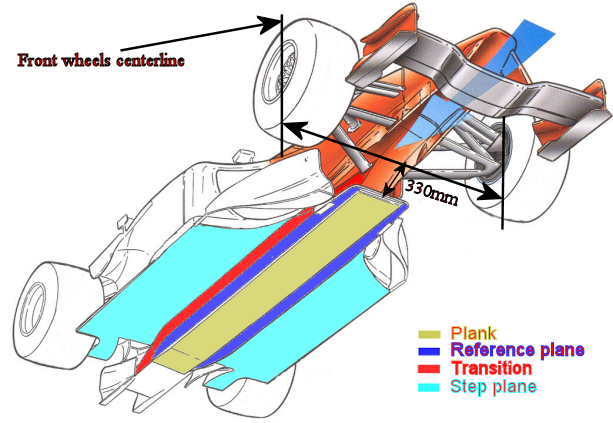
\includegraphics[height=4.8cm]{Figures/undertray_f1.png}
  \end{subfigure}
%  
  \caption{Typical undertray of a formula race-car \cite{Katz1995RaceSpeed}\cite{AnonymousUndertrayUnderbody}}
    \label{fig:underbody}
\end{center}
\end{figure}

\noindent As stated before, the concept of Venturi tunnel is used for an undertray to generate downforce. the convergent section of the Venturi tunnel allows the increase in velocity which reduce the pressure on the floor section. A significant pressure reduction create a suction-like phenomena which push the car down and create a higher traction. On the rear side of the undertray is the divergent section (diffuser) where kinetic energy is converted into a pressure rise. 
\noindent Up to QFR 2021, undertray is the only passive aerodynamics device which will be produced and attached to the car. The development of undertray of QFR 2021 has been done previously in 2017 \cite{McKeown2018DesignCar} and 2019 \cite{McClune2018DesignCar}. The work has included a numbers of 2D simulations which tested various variables of the undertray such as diffuser and inlet angle, as well some of 3D undertray. The case analyses by McKeown \cite{McKeown2018DesignCar} and McClune \cite{McClune2018DesignCar} was flawed due to the non-existence of bluff body. This allows the analysis on the undertray force generation affected by the flow acting on the top of the undertray which makes the analyses unrealistic to the real-life situation \cite{Corr2017MechanicalAuthor}. Therefore this paper will dig deeper on the flow behaviour of the underbody with bluff body both on 2D and 3D analyses. 

\subsubsection{Undertray Devices}
The geometry design of an undertray is strictly regulated by the competition. Although Formula students rules is more flexible, there are some device implementation in formula car that could slightly improve the aerodynamics performance. Such devices are diffuser fences and Gurney flaps.

\begin{figure}[!ht]
\begin{center}
%    
  \begin{subfigure}[b]{0.4\textwidth}
    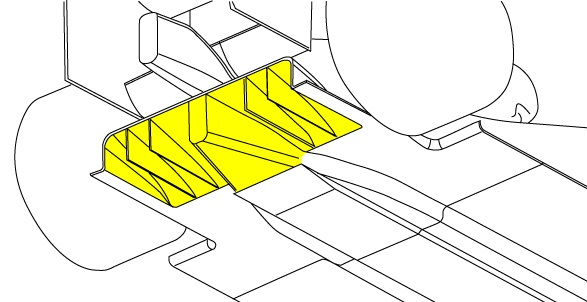
\includegraphics[scale=0.6]{Figures/diffuser_fences.jpg}
  \end{subfigure}
  %
  \begin{subfigure}[b]{0.4\textwidth}
    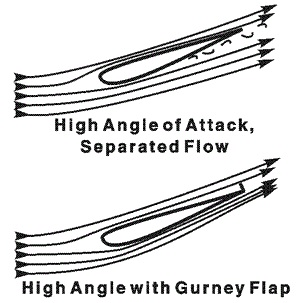
\includegraphics[scale=0.8]{Figures/Gurney.jpg}
  \end{subfigure}
%  
  \caption{Fences or strake on a diffuser(left) and example of a Gurney flap application on a wing (right) \cite{Anonymous2020GurneyFlap}.}
    \label{fig:gurney}
\end{center}
\end{figure}

\noindent Fence or strake on a diffuser acts as a force generator. As discussed previously, the corner vortices occurred at rear diffuser generates downforce and strake helps the diffuser to generate more than two vortices hence increase more downforce. Figure \ref{fig:gurney} left shows the example of a basic strake on a diffuser. Gurney flap is an small flap or L-shape structure attached at the end of diffuser which shown in figure \ref{fig:gurney} right. Generally, Gurney flap is used to improve downforce without significant drag \cite{Willemsen2012CFD-basedDiffuser} by making the boundary layer stay attached and delay flow separation to the end of diffuser by reducing the pressure on the underside of diffuser and increasing the pressure on the top of diffuser. 

\noindent Despite the advantageous function of both device, there are still lack of information provided in this area hence further analysis will be a good leap in improving an undertray performance.  
